\chapter{Krav}
Dette afsnit har til formål at beskrive, hvilke krav der er til systemet, og skabe et overordnet overblik over rammerne for systemet. \\
Med udgangspunkt i projektformuleringen, er der udarbejdet seks Use Cases, som repræsenterer de funktionelle krav for systemet. Hver Use Case dækker over et givet krav og beskriver brugerens interaktion med systemet. Samlet dækker de seks Use Cases over systemets funktionalitet.\\
Systemets primære funktionalitet beskrives ved UC2, UC6, samt enkelte ikke-funktionelle krav, der tydeliggør muligheden for at monitorere et kontinuerligt blodtryk på en computerskærm, og gemme en måling til efterfølgende forskning.

\begin{figure}[H]
	\centering
	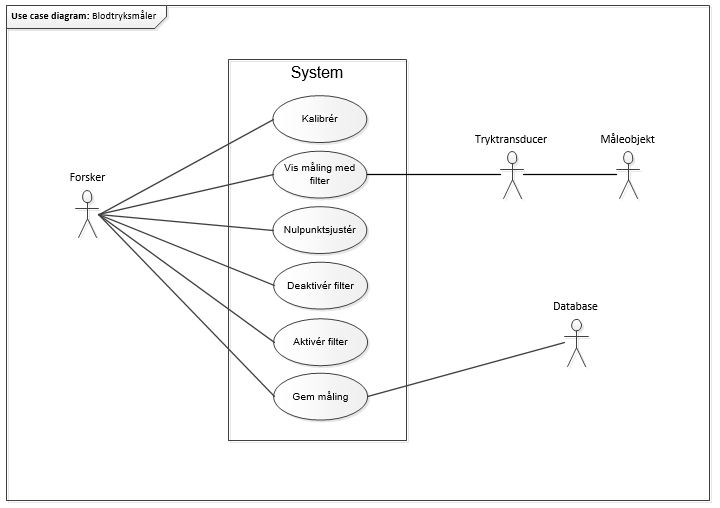
\includegraphics[width=1\textwidth]{Figurer/1}
	\caption{Use Case diagram}
\end{figure}

Ovenfor ses de funktionelle krav beskrevet ud fra et Use Case diagram, der samtidig viser, hvilke aktører, der har betydning for hvilke Use Cases.  Aktører beskrives herunder:
\\\\

\textbf{Forsker} er den primære aktør for samtlige seks Use Cases, hvilket betyder at forskeren initierer alle Use Cases og dermed styrer programmet og dets funktioner. Forskeren sidder med den fulde kontrol over systemet, og kan bestemme hvad der skal ske og hvornår.
\\\\
\textbf{Måleobjekt} er sekundær aktør i UC2 og det er her blodtrykket måles på. Måleobjektet kan enten realiseres in vivo eller in vitro.
\\\\
\textbf{Tryktransducer} er sekundær aktør i UC2 og fungerer som et bindeled mellem de to aktører, Forsker og Måleobjekt. Den sørger for, at omforme det målte tryk fra Måleobjektet om til et analog signal, som systemet kan behandle og fremvise på brugervenlig form for Forskeren. 
\\\\
\textbf{Database} er sekundær aktør i UC6 og den er ansvarlig for at blodtryksmålinger kan gemmes.
\\\\
Nedenfor ses en kort beskrivelse af de seks Use Cases og aktørernes roller i disse. For yderligere detaljer af Use Cases henvises til kravspecifikationen i projektdokumentationen.
\\\\
\textbf{UC1: Kalibrér}\\
Forskeren skal kunne kalibrere systemet via en grafisk brugergrænseflade.
\\\\
\textbf{UC2: Vi måling med filter}\\
Forskeren skal kunne se en kontinuerlig blodtrykskurve for et givet måleobjekt på en grafisk brugergrænseflade. 
\\\\
\textbf{UC3: Nulpunktsjustér}\\
Forskeren skal kunne nulpunktsjustere systemet via en grafisk brugergrænseflade.
\\\\
\textbf{UC4: Deaktivér filter}\\
Forskeren skal kunne deaktivere det digitale filter og udskrive det ufiltrerede blodtrykssignal på en grafisk brugergrænseflade.
\\\\
\textbf{UC5: Aktivér filter}\\
Forskeren skal kunne aktivere det digitale filter og udskrive det filtrerede blodtrykssignal på en grafisk brugergrænseflade.
\\\\
\textbf{UC6: Gem måling}\\
Forskeren skal kunne optage blodtryksmålinger og derefter gemme dem i en Database. 
\\\\
Udover de funktionelle krav, er der vha. FURPS+ opstillet en række ikke-funktionelle krav med henblik på at klarlægge design og kvalitetsgrad for systemet. \\
Herunder bliver der beskrevet krav til bl.a. design af den grafiske brugergrænseflade, systemets præstation og diverse krav til udstyr og generel  af udvikling af systemet.\\
Det er gældende for hele den grafiske brugergrænseflade, at alle knapper skal være selvforklarende i forhold til den funktion, de varetager. Det gælder bl.a. knapperne ”Beregn”, ”Nulpunktsjuster”, ”Rec”, ”Stop” og ”Gem”.\\
Ydermere er der forsøgt, at overholde diverse standarder for design af en grafisk brugergrænseflade, hvad angår placering, størrelse og farve af knapper, værdier, grafer mv.\\
For yderligere detaljer af ikke-funktionelle krav henvises der til kravspecifikationen i projektdokumentationen.



 



